\documentclass[border=5pt]{standalone}
\usepackage{tikz}
\usetikzlibrary{shapes,arrows,positioning,fit,backgrounds,calc,chains}

\begin{document}

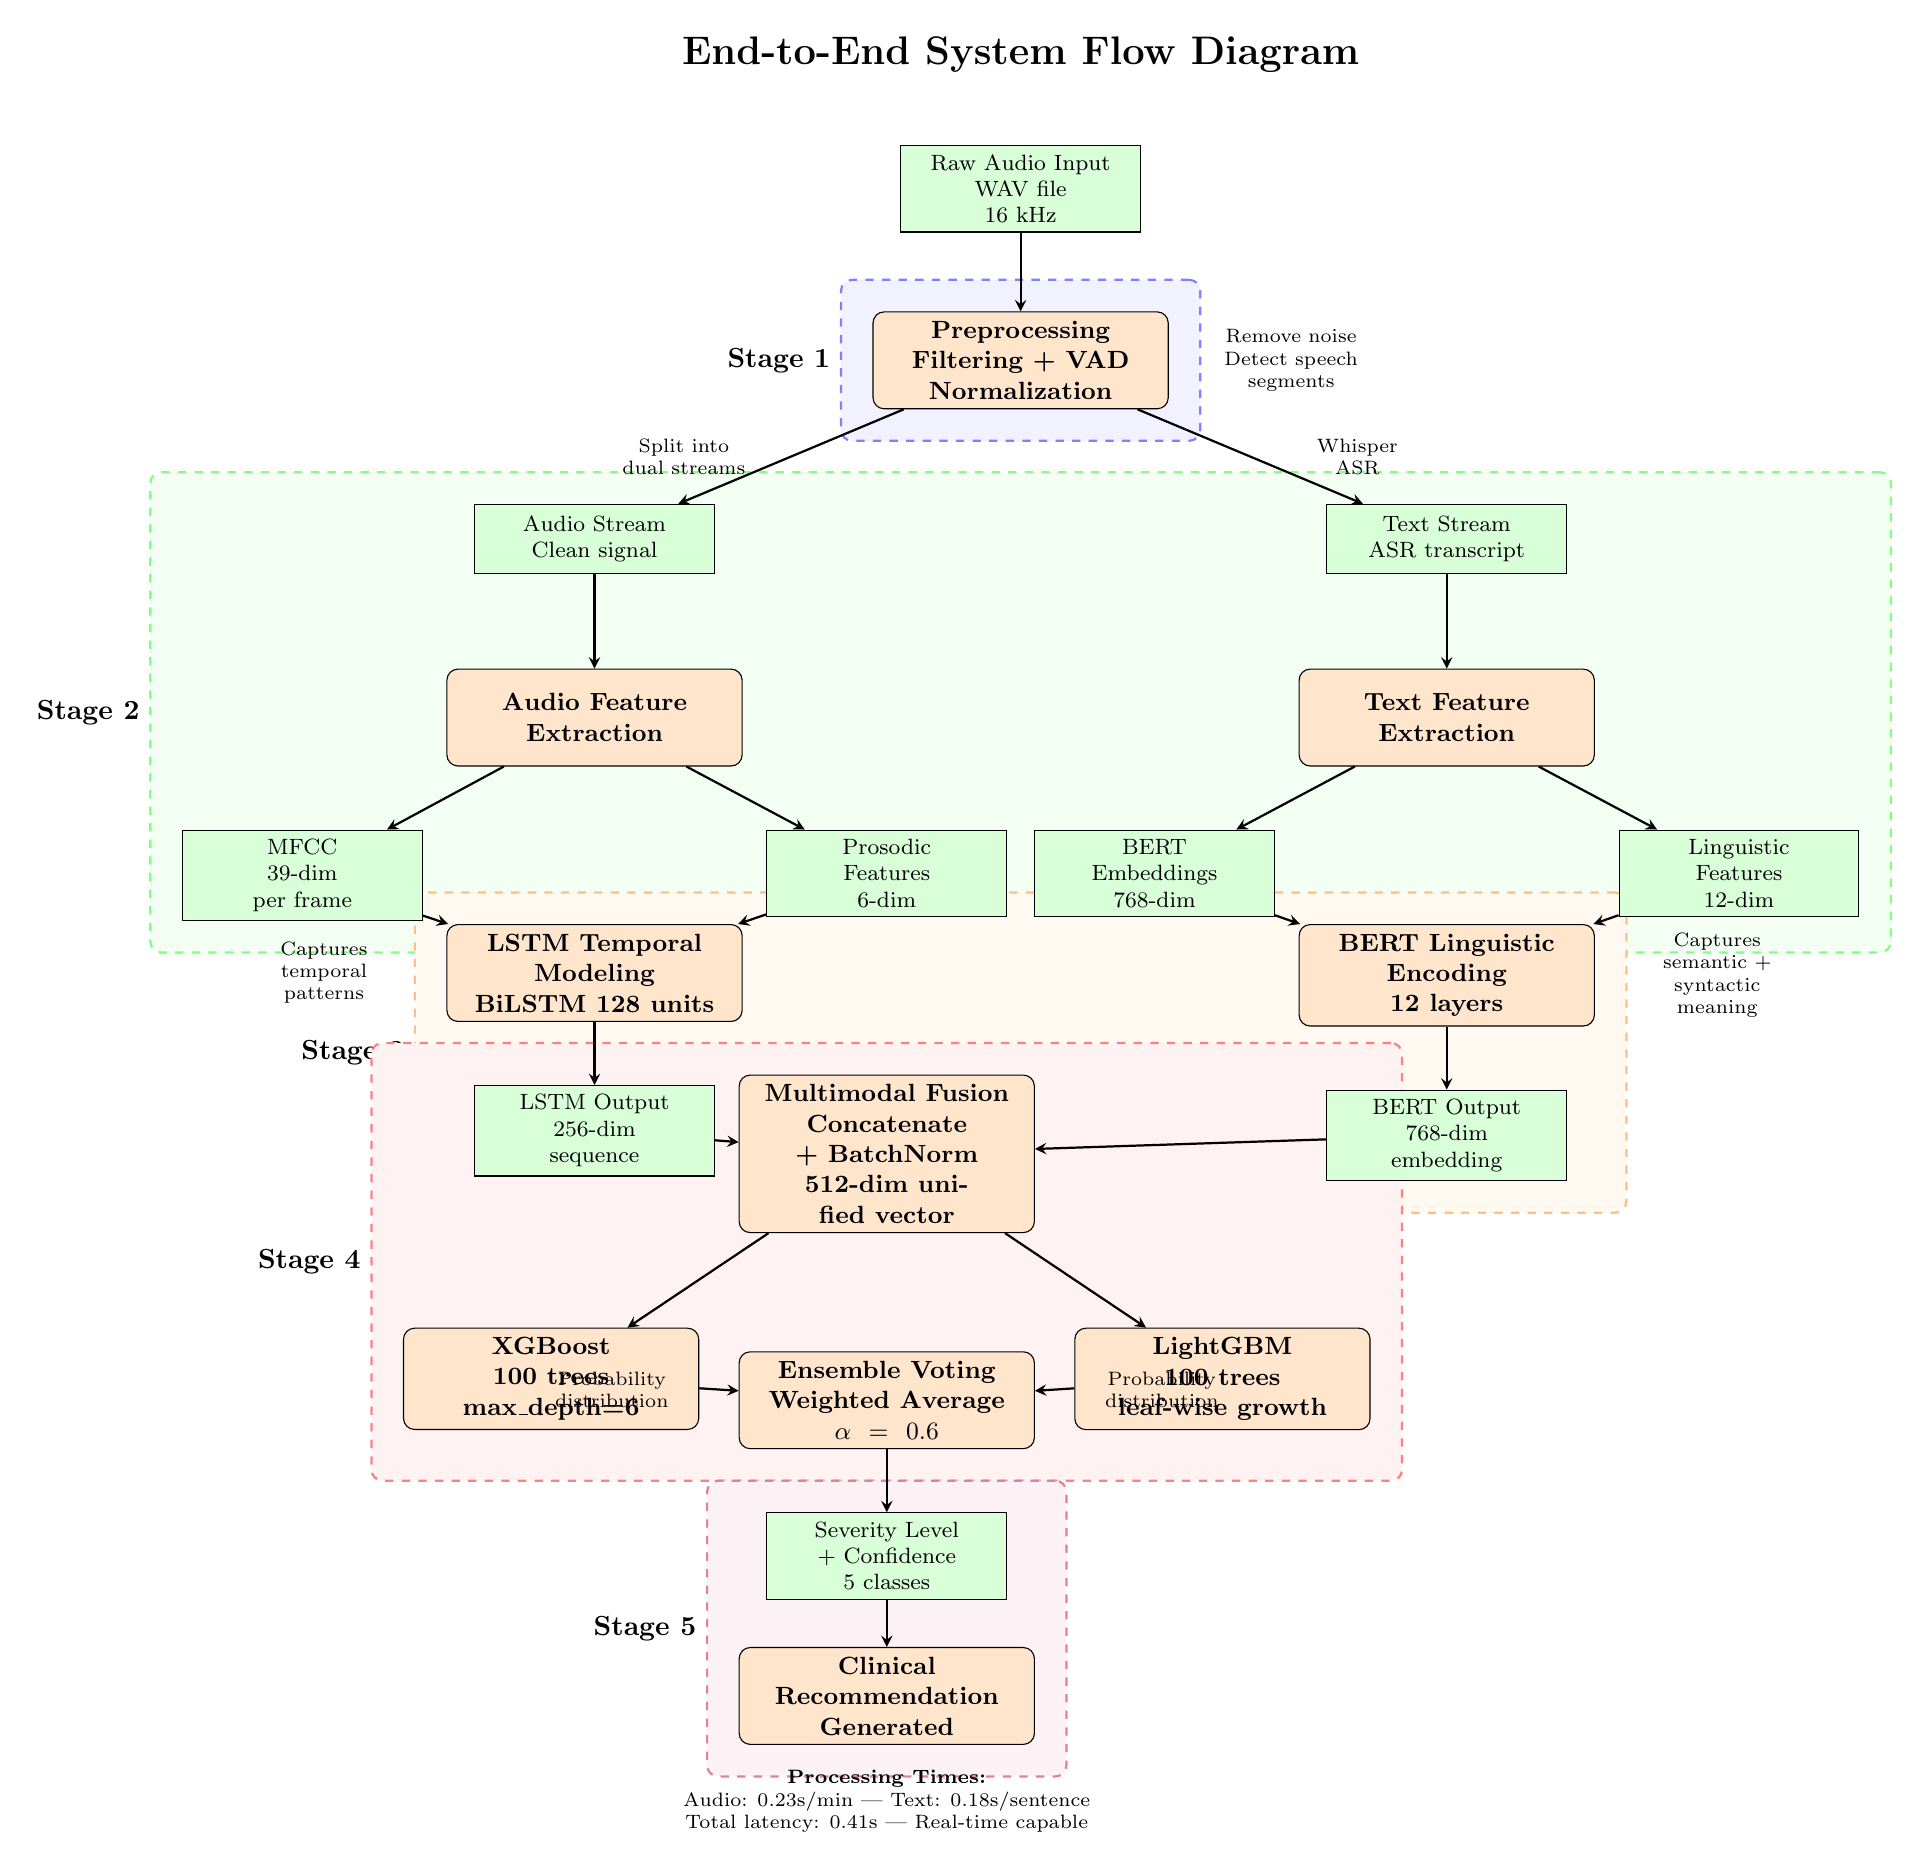
\begin{tikzpicture}[
    node distance=1cm and 1.5cm,
    box/.style={rectangle, draw, fill=blue!15, text width=9em, text centered, rounded corners, minimum height=3em, font=\small},
    databox/.style={rectangle, draw, fill=green!15, text width=8em, text centered, minimum height=2.5em, font=\footnotesize},
    processbox/.style={rectangle, draw, fill=orange!20, text width=10em, text centered, rounded corners, minimum height=3.5em, font=\small\bfseries},
    arrow/.style={thick,->,>=stealth},
    doublearrow/.style={thick,<->,>=stealth},
    annotation/.style={font=\scriptsize, text width=7em, align=center}
]

% Top: Raw Input
\node [databox] (rawinput) {Raw Audio Input\\WAV file\\16 kHz};

% Preprocessing Stage
\node [processbox, below=of rawinput] (preproc) {Preprocessing\\Filtering + VAD\\Normalization};

\node [annotation, right=0.2cm of preproc] {Remove noise\\Detect speech\\segments};

% Dual Stream Split
\node [databox, below left=1.2cm and 2cm of preproc] (audio_stream) {Audio Stream\\Clean signal};
\node [databox, below right=1.2cm and 2cm of preproc] (text_stream) {Text Stream\\ASR transcript};

% Audio Feature Extraction
\node [processbox, below=1.2cm of audio_stream] (audio_feat) {Audio Feature\\Extraction};

\node [databox, below left=0.8cm and 0.3cm of audio_feat] (mfcc_data) {MFCC\\39-dim\\per frame};
\node [databox, below right=0.8cm and 0.3cm of audio_feat] (pros_data) {Prosodic\\Features\\6-dim};

% Text Feature Extraction
\node [processbox, below=1.2cm of text_stream] (text_feat) {Text Feature\\Extraction};

\node [databox, below left=0.8cm and 0.3cm of text_feat] (bert_data) {BERT\\Embeddings\\768-dim};
\node [databox, below right=0.8cm and 0.3cm of text_feat] (ling_data) {Linguistic\\Features\\12-dim};

% Deep Learning Analysis
\node [processbox, below=2cm of audio_feat] (lstm_model) {LSTM Temporal\\Modeling\\BiLSTM 128 units};

\node [processbox, below=2cm of text_feat] (bert_model) {BERT Linguistic\\Encoding\\12 layers};

\node [annotation, left=0.2cm of lstm_model] {Captures\\temporal\\patterns};
\node [annotation, right=0.2cm of bert_model] {Captures\\semantic +\\syntactic\\meaning};

% Feature outputs
\node [databox, below=0.8cm of lstm_model] (lstm_out) {LSTM Output\\256-dim\\sequence};
\node [databox, below=0.8cm of bert_model] (bert_out) {BERT Output\\768-dim\\embedding};

% Multimodal Fusion
\node [processbox, below=2cm of pros_data] (fusion) {Multimodal Fusion\\Concatenate + BatchNorm\\512-dim unified vector};

% Ensemble Classification
\node [processbox, below left=1.2cm and 0.5cm of fusion] (xgb_model) {XGBoost\\100 trees\\max\_depth=6};

\node [processbox, below right=1.2cm and 0.5cm of fusion] (lgbm_model) {LightGBM\\100 trees\\leaf-wise growth};

% Ensemble Voting
\node [processbox, below=1.5cm of fusion] (voting) {Ensemble Voting\\Weighted Average\\$\alpha = 0.6$};

% Final Output
\node [databox, below=0.8cm of voting] (severity_out) {Severity Level\\+ Confidence\\5 classes};

\node [processbox, below=0.6cm of severity_out] (clinical) {Clinical\\Recommendation\\Generated};

% Draw arrows with labels
\draw [arrow] (rawinput) -- (preproc);
\draw [arrow] (preproc) -- node[left, annotation] {Split into\\dual streams} (audio_stream);
\draw [arrow] (preproc) -- node[right, annotation] {Whisper\\ASR} (text_stream);

% Audio path
\draw [arrow] (audio_stream) -- (audio_feat);
\draw [arrow] (audio_feat) -- (mfcc_data);
\draw [arrow] (audio_feat) -- (pros_data);
\draw [arrow] (mfcc_data) -- (lstm_model);
\draw [arrow] (pros_data) -- (lstm_model);
\draw [arrow] (lstm_model) -- (lstm_out);

% Text path
\draw [arrow] (text_stream) -- (text_feat);
\draw [arrow] (text_feat) -- (bert_data);
\draw [arrow] (text_feat) -- (ling_data);
\draw [arrow] (bert_data) -- (bert_model);
\draw [arrow] (ling_data) -- (bert_model);
\draw [arrow] (bert_model) -- (bert_out);

% Fusion path
\draw [arrow] (lstm_out) -- (fusion);
\draw [arrow] (bert_out) -- (fusion);

% Ensemble path
\draw [arrow] (fusion) -- (xgb_model);
\draw [arrow] (fusion) -- (lgbm_model);
\draw [arrow] (xgb_model) -- node[left, annotation] {Probability\\distribution} (voting);
\draw [arrow] (lgbm_model) -- node[right, annotation] {Probability\\distribution} (voting);

% Output path
\draw [arrow] (voting) -- (severity_out);
\draw [arrow] (severity_out) -- (clinical);

% Background stages
\begin{scope}[on background layer]
    \node[draw=blue!50, thick, dashed, rounded corners, fit=(preproc), fill=blue!5, inner sep=0.4cm, label=left:\textbf{Stage 1}] {};
    
    \node[draw=green!50, thick, dashed, rounded corners, fit=(audio_stream)(text_stream)(audio_feat)(text_feat)(mfcc_data)(pros_data)(bert_data)(ling_data), fill=green!5, inner sep=0.4cm, label=left:\textbf{Stage 2}] {};
    
    \node[draw=orange!50, thick, dashed, rounded corners, fit=(lstm_model)(bert_model)(lstm_out)(bert_out), fill=orange!5, inner sep=0.4cm, label=left:\textbf{Stage 3}] {};
    
    \node[draw=red!50, thick, dashed, rounded corners, fit=(fusion)(xgb_model)(lgbm_model)(voting), fill=red!5, inner sep=0.4cm, label=left:\textbf{Stage 4}] {};
    
    \node[draw=purple!50, thick, dashed, rounded corners, fit=(severity_out)(clinical), fill=purple!5, inner sep=0.4cm, label=left:\textbf{Stage 5}] {};
\end{scope}

% Title
\node[above=0.8cm of rawinput, font=\Large\bfseries] {End-to-End System Flow Diagram};

% Processing time annotations
\node[below=0.2cm of clinical, font=\scriptsize, align=center] {
    \textbf{Processing Times:}\\
    Audio: 0.23s/min | Text: 0.18s/sentence\\
    Total latency: 0.41s | Real-time capable
};

\end{tikzpicture}

\end{document}
